\ifgerman{\chapter{Auswertung}}{\chapter{Implementation}}
\label{sec:implementation}

\section{Simulation Environment}

The FINken consists of the body, the rotors and the sensors. The body contains the behavioural and flight control, the thrust simulation is handled by scripts connected to the rotor structure.

\subsection{Scene Modeling}

The body consists of multiple objects, while visual representation and the physical behaviour are split. For visual representation, a *.stl file from the CAD-Model of the original FINken was imported. This shape is rather complex, which makes the simulation time consuming. To speed up the simulation, the shape of the finken was remodelled in VREP, using only simple rectangular shapes. Making the complex shape static, establishing a fixed connection and hiding the simple shape, the result is a a visual appealing simulation object with good simulation performance. A dummy-object is used as a singular measurement reference point in the middle of the FINken. This has to be taken into account when targeting physical objects, as the FINken will not be able to reach the target completely without colliding with the object. This dummy object should always be used when refering to the FINkens position, orientation or movements, as it is aligned to the global coordinate system while especially imported shapes may be rotated in the simulation.
\begin{figure}[h!]
 \begin{center}
  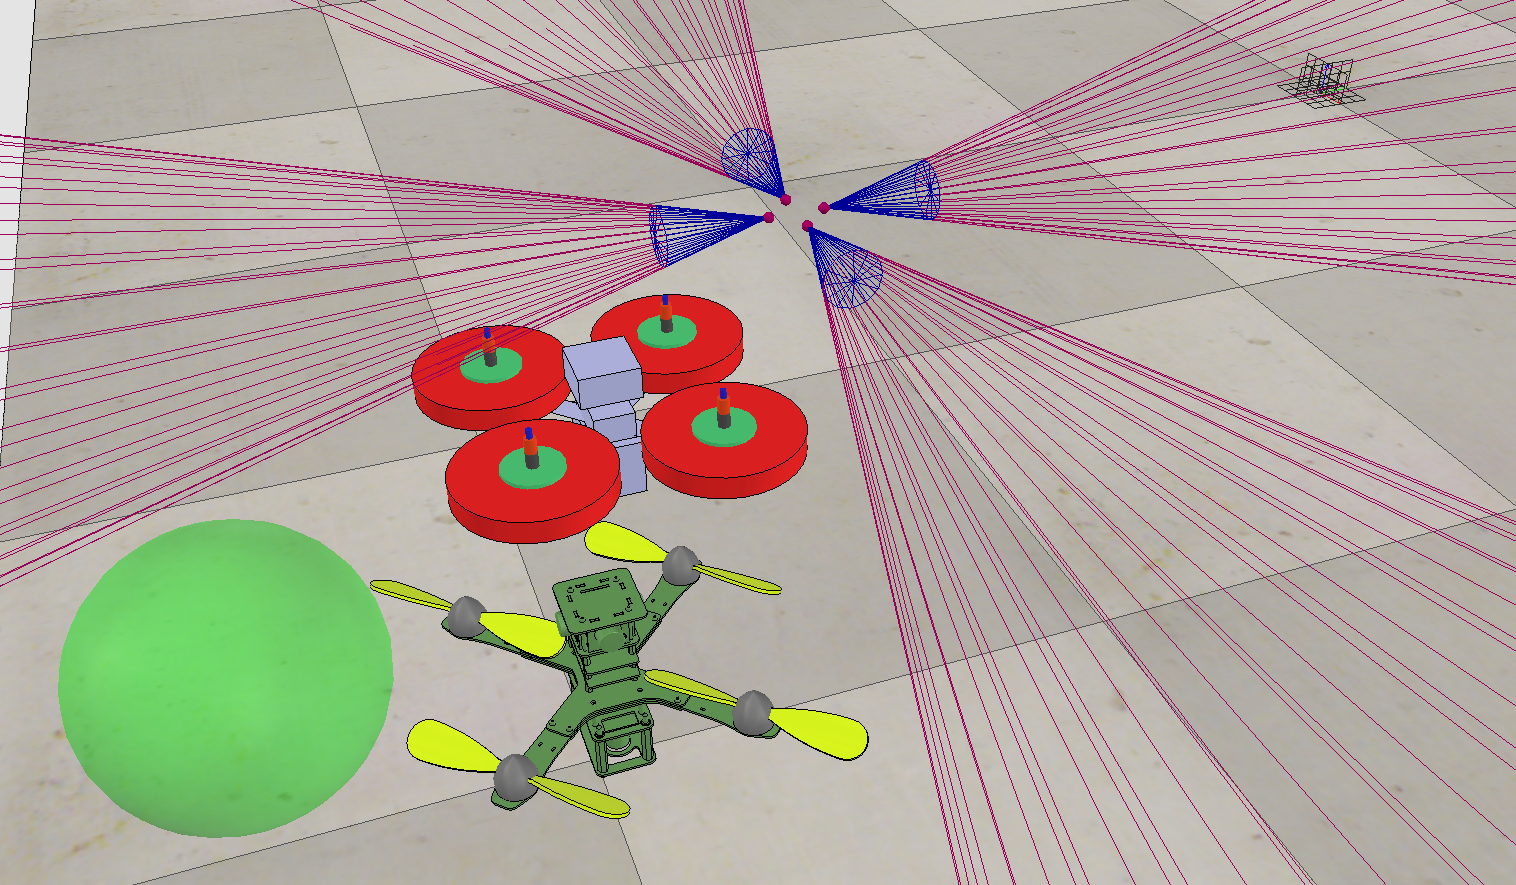
\includegraphics[width=\linewidth]{vrepDisassemlbyFull.png}
 \end{center}
  \caption{Parts of the simulation object \label{fig:vrepParts}}
\end{figure}
The measured weight of the real FINken was applied to the simulation object. As no advanced modelling like calculating moments of inertia was done, the weight of the motor was applied separately to the rotor model in VREP.  The motor assembly adds significant weight outside the FINkens center of gravity and therefore has a rather large influence on its behaviour. 
\todo{weight table for finken2 and finken3}
The linear damping factor of the FINken body material was set to 0.3, to decrease drift and to model the air resistance of the real FINken, which is minimal but nevertheless existent.


The rotor model in VREP handles the thrust simulation and thus a huge part of the physical behaviour of the quadcopter model.  Again, visual representation and physical simulation are separated. 
\todo{add picture of rotor}
The visualisation is done with a static shape of a rotor, that is connected to a joint and rotates with a fixed speed. During flight, the rotation speed does not really change visually noticeable, a dynamic adaption of the rotation would only increase computation time without much benefit. Of course, the rotor shape could be made non-static and rotate in a particle stream, and apply the thrust force according to the particle collisions, but again, this would mean a massive increase of computation power and is not needed for our purposes.
\todo{picture of rotor simulation and rotor visualisation}
he rotor model is attached to the FINken body via a force sensor which applies the forces and torques calculated in the physical rotor model to the FINken body. The rotor is represented by a cylindrical shape which resembles the area swept by a real rotor and uses a particle simulation to emulate the airstream. The handling of the particle simulation is done inside a lua child script attached to the rotor model. The script has several parameters for the particle simulation, \todo{add complete param list}.
During simulation, the particle velocity is the parameter used to control the finken. 
\todo{add formula to show linearity between thrust and airstream velocity} 


Vrep provides several physics engines, we use the default bullet engine for our simulation.

\subsection{Simulation Software Structure}

The simulation software is written in Lua and runs inside a non-threaded child script of each FINken quadrocopter in VREP.  

The base class is the finkenCore, which contains the main flight control algorithm and a steering interface as well as an interface to the FINkens sensors.
The input commands for controlling the FINken are set via the signal communication of VREP. Signals inside VREP are the most versatile communication possibility which can be accessed from anywhere inside VREP and any remote API, they can be seen as a kind of global variable. Signals can be of integer, float or string type, where custom data types can be sent in text form as string signals. 


\todo{diagram of finken software}

\todo{finken parameter estimation}

\todo{controller tuning}

\todo{simulation parameters}

\todo{script structure}


\section{Communication V-REP - Quadrocopters}
\label{sec:commImplementation}

This chapter describes the implementation of the requirements on the Java-API, which ware discussed in \ref{sec:communication} of \ref{chap:theo}. It begins with an overview of the software architecture and continues with the explanation of the created projects, classes and their use. It helps understanding how the communication between the V-REP and the quadrocopters is implemented and how to use the API or extend it in order to implement other mixed-reality scenarios.\\
Note that this is just a brief explanation of the Java-API implementation. If you want to go in details refer to the Javadoc which is also provided as an attachment to this paper.

\subsection{Software architecture}

The software architecture of the Java-API, which serves as a communication bridge between the Paparazzi software and the V-REP simulation, is designed to be as modular as possible in order to facilitate the further development of the project. Its reusable components should also serve as a building blocks for the students that want to develop future mixed-reality projects. \\

On \ref{fig:apiArchitecture} is depicted an raw overview of the Java-API software architecture.
The final program is assembled from independently developed components. Each part is independent and provide well-defined exported interfaces so that the other parts can use them.
The first layer contains the projects \textit{JavaV-REP}, \textit{JavaIvyBus} and \textit{JavaXmlSax}.\\
The \textit{JavaV-REP} is the implementation of the requirements concerning V-REP, that ware discussed in \ref{sec:requirementsVREP} of \ref{chap:theo}. At the heart of this project is the V-REP Remote-API binding for Java provided by Coppelia. The \textit{JavaVrep} project extends this library and provides further utility methods for establishing connection to remote V-REP servers as well as retrieving and manipulating scene objects. The \textit{JavaV-REP} project is described in more details in \ref{sec:vrepImplementation}.\\

\begin{figure}[h!]
 \begin{center}
  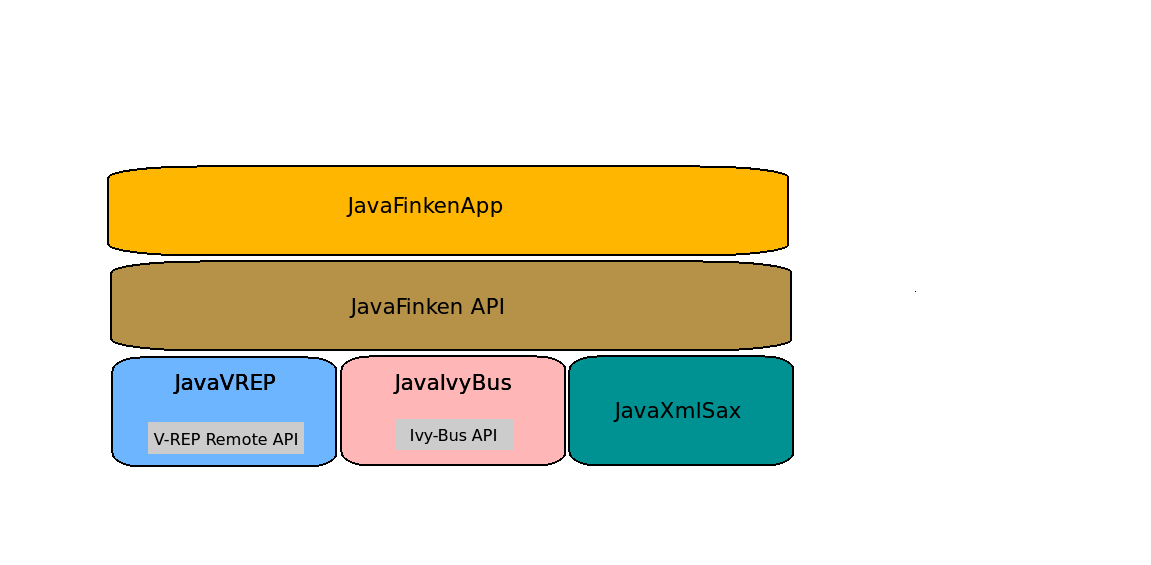
\includegraphics[scale=0.6]{apiArchitecture.png}
 \end{center}
  \caption{Java-API architecture\label{fig:apiArchitecture}}
\end{figure}

\textit{JavaIvyBus} is a Java project, that imports the Ivy-Bus library and implements the requirements regarding Ivy-Bus, which ware discussed in \ref{sec:requirementsIVYBus}.\\ 
It extends the functionality of the the Ivy-Bus library and provides the programmer with the possibility to create Ivy-Bus nodes by just instantiating an object which takes as constructor parameter the name of the bus-node. It facilitates the connection or disconnection from the bus by just calling a function the the created bus-node object. The abstractions on which this project rely also allow to easily create bus messages or just parse them from xml file and subscribe to them even dynamically. The \textit{JavaIvyBus} project is discussed in more detail in \ref{sec:ivyBusImplementation}. \\

The \textit{JavaXmlSax} project is a small API, that allows the programmer to easily create a custom xml reader that parses any xml document and retrieves the instances of the objects defined by the xml. It consists of several abstract classes, that provide the template for the custom xml readers.\\
A short explanation of how this API can be used is included in \ref{sec:xmlImplementation}. \\

On the next layer in the hierarchy is the \textit{JavaFinken} API. It uses the APIs from the layer below to provide further abstractions and utilities for our FINKEN project. It consists of classes that describe 
the aircrafts defined in the paparazzi, defines the basic classes that represent our virtual and real quadrocopters and their sensors, defines a representation of the telemetry and the V-REP signals. With the help of \textit{JavaIvyBus} API, lying on the layer below, the Ivy-Bus nodes, specific for the virtual and real quadrocopters are represented. The abstraction provided by \textit{JavaXmlSax} is used to create a custom Xml readers for parsing the telemetry, messages and aircrafts from the Xml files. A more detailed description of the API is included in \ref{sec:javaFinkenImplementation} \\

On the top of the hierarchy is situated the actual application of our project called \textit{JavaFinkenAPP}. It uses \textit{JavaFinken} API to bind the provided utility classes in a specific application meeting our project requirements. The application has a simple Graphical User Interface that facilitates specifying the IP and Port number of the V-REP simulation server, specifying path to the paparazzi software, a button for establishing the connection and other UI elements.




\subsection{JavaV-REP}
\label{sec:vrepImplementation}

All the functionality, that concerns V-REP and was discussed in \ref{sec:requirementsVREP} of \ref{chap:theo} is implemented as a single Java project called \textit{JavaVREP}.\\
 The project uses the V-REP Remote-API Java binding - package \textit{coppelia} (containing 12 Java classes) and the \textit{libremoteApiJava.so} or \textit{libremoteApiJava.dll} (depending if the platform is Linux or Windows). The \textit{libremoteApiJava.so} should be placed in the Java home directory, e.g \textit{/usr/lib/jvm/java-8-oracle/jre/lib/amd64}, in order for the project to be compiled.\\
The main class is the \textit{VrepConnection.java}, which is a wrapper of the \textit{remoteApi.java} class provided by the V-REP remote API. Its singleton instance can be retrieved by calling:

\begin{center}
\begin{tabular}{c}
\begin{lstlisting}[basicstyle=\small]
VrepConnection connection = VrepConnectionUtils.getConnection();
\end{lstlisting}
\end{tabular}
\end{center}

The above expression loads the remote API library and returns the instance of \textit{VrepConnection} on which the Remote API functions are called. For example to retrieve all objects in a scene the following function have to be called on the \textit{VrepConnection} instance:

\begin{center}
\begin{tabular}{c}
\begin{lstlisting}[basicstyle=\small]

connection.simxGetObjects();

\end{lstlisting}
\end{tabular}
\end{center}

The interfaces \textit{VrepServer} and \textit{VrepClient} and their implementations \textit{StandardVrepServer} and \textit{StandardVrepClient} describe the two end-points of the communication. The \textit{VrepServer} describes the IP address and the port number of the machine on which the V-REP is running. In order to connect to a V-REP server we have to create in instance of the \textit{VrepServer} and open the client:

\begin{center}
\begin{tabular}{c}
\begin{lstlisting}[basicstyle=\small, language=Java]
VrepConnection connection;
VrepClient     client;
VrepServer     server;

connection = VrepConnectionUtils.getConnection();
client     = VrepClientUtils.getClient();
server     = new StandardVrepServer("127.0.0.1", "19999");

client.connectToServer(server);

if (!client.isConnected()) {
// error in connection
} 
\end{lstlisting}
\end{tabular}
\end{center}

The above example shows how to connect to a V-REP server. The IP \textit{127.0.0.1} specifies that the server is running on the same machine. The port number can be chosen arbitrary, but have to match on both client and server site.\\
In order to close the connection just the method \textit{client.close()} has to be called. \\

The \textit{VrepClient} conforms to the Java Beans specification and can thus fire events when the connection has been established or disconnected. Any class who is interested in catching these events asynchronously, for example GUI, will have to implement \textit{PropertyChangeListener} and register. See
\url{https://docs.oracle.com/javase/tutorial/javabeans/writing/events.html} for more information. \\

Each V-REP scene object is represented by the interface \textit{VrepObject} and the \textit{AbsVrepObject} represents an abstract scene object from which all types of object derive. The abstract scene object has private properties like \textit{Position}, \textit{Orientation}, \textit{LinearVelocity} and \textit{AngularVelocity}, which represent its inertial parameters taken from the V-REP.
\textit{VrepObjectType} is an Enum, that specifies the scene object type like Shape, Path, Proximity sensor etc. The name of the scene object is represented by the class \textit{VrepObjectName}, which consists of a base name and an index. If an object is copy-pasted (multiple instances of an object), then
each instance of the object receives the following name, according to V-REP naming scheme: \textit{\texttt{base\_name\#index}}. For example if we want to have three quadrocopters, their names in V-REP will be represented as follows: \textit{\texttt{Quad\_Lia\_ovgu\_01}}, \textit{\texttt{Quad\_Lia\_ovgu\_02\#0}} and \textit{\texttt{Quad\_Lia\_ovgu\_03\#1}}. \\

The V-REP scene is represented by the class \textit{VrepScene}, which retrieves all objects and hold a collection of them for further use. Since we always have one V-REP scene the class is designed as a Singleton pattern. The following example shows how this class is used for loading the scene and retrieving all shape objects.

\begin{center}
\begin{tabular}{c}
\begin{lstlisting}[basicstyle=\small, language=Java]
VrepScene   scene;
List<Shape> shapeObjects;

scene = VrepSceneUtils.getVrepScene();
scene.loadScene();
shapeObjects = scene.getAllShapeObjects();

\end{lstlisting}
\end{tabular}
\end{center}

The project \textit{JavaVrep} also defines the interface \textit{ObjectUpdator} and its abstract implementation \textit{AbsObjectUpdator}, which is used to update the \textit{VrepObject}s with real-time parameters from V-REP, like their \textit{Position}, \textit{Orientation}, \textit{LinearVelocity} and \textit{AngularVelovity}.


\subsection{JavaIvyBus}
\label{sec:ivyBusImplementation}

The requirements regarding the Ivy-Bus, that ware stated in \ref{sec:requirementsIVYBus} of \ref{chap:theo} are implemented in a stand-alone Java project called \textit{JavaIvyBus}. \\
The project requires the \textit{ivy-java.jar} library to be on its class path in order to be compiled.\\
The project contains class definitions of the Paparazzi messages that are defined in a Xml file. See listing \ref{lst:MessageXml} of \ref{chap:theo}. The interface \textit{Message} and its abstract implementation \textit{AbsMessage} describe such a message with its name, period at which the message is sent, identifier and \textit{MessageField}s. \\
The interface \textit{IvyBusNode} represents a single independent node communicating on the common bus. By inheriting from its abstract implementation \textit{AbsIvyBusNode}, one can create a custom bus-node. The methods \textit{IvyBusNode.connect()} and \textit{IvyBusNode.disconnect()} are used to attach the particular node to the bus and disconnect it. The \textit{IvyBusNode} also conforms to the Java Beans specification and and fires asynchronous notifications each time the node joins or leaves the bus.
After obtaining an instance of a \textit{Message}, parsed from the Xml file or a custom-created, the bus-node can subscribe to this \textit{Message} by invoking the method \textit{IvyBusNode.subscribeToMessage(Message msg)} and thus receive all the messages of this kind or use the method \textit{IvyBusNode.subscribeToIdMessage(Message msg, int id)}, which subscribes to the messages published just by this quadrocopter ehich has the same id. \\
Once a \textit{Message} to which the bus node has subscribed has been received, the bus node fires an notification and gives the instance of the received \textit{Message}, with all of its \textit{MessageField}s initialized with the actual message values. The following listing shows an example hot to subscribe to a message and get asynchronous notification when the message is received.

\begin{center}
\begin{tabular}{c}
\begin{lstlisting}[basicstyle=\small, language=Java]

class TestBusNode implements PropertyChangeListener {
  
  private IvyBusNode node; 
  private Message    message;
  
  public TestBusNode(IvyBusNode node, Message msg) {
    this.node    = node;
    this.message = msg;
    
    this.node.addPropertyChangeListener(this);
    this.node.subscribeToMessage(this.message);
  }
  
  @override
  public void propertyChange(PropertyChangeEvent event) {
    Message receivedMessage;
    
    // the message has been received
        
    receivedMessage = (Message)event.getNewValue();    
  }

}

\end{lstlisting}
\end{tabular}
\end{center}


\subsection{JavaXmlSax}
\label{sec:xmlImplementation}

\subsection{JavaFinken}
\label{sec:javaFinkenImplementation}

The \textit{JavaFinken} API is a project that relies on the previously introduces projects \textit{JavaV-REP}, \textit{JavaIvyBus} and \textit{JavaXmlSax}. It provides the basic classes and utilities upon which our application can be built.

\section{\todo{fancy name }}

\section{Quadcopter}



% example for bar plots
%\begin{tikzpicture}
%  \centering
%  \begin{axis}[
%        ybar = 0,
%    height=6cm,
%    width=15cm,
%    enlarge x limits={rel=0.1},
%    axis lines*=left,
%    ymin=0,
%    ymax=50,
%     legend style={at={(0.5,-0.27)},
%        anchor=north,legend columns=-1},
%        ylabel={\#Anzahl Blöcke},
%        xlabel={Halstead Volumen},
%        cycle list = {black,black!70,black!40,black!10},
%        symbolic x coords={10,20,30,40,50,70,90,120,300,750,>750},
%     xtick=data,
%        nodes near coords,
%    every node near coord/.append style={
%        anchor=mid west,
%        rotate=90 }]
%     \addplot+[] coordinates {(10,3) (20,18) (30,8)(40,1)(50,0)(70,6)(90,6)(120,0)(300,2)(750,0)(>750,0)};
%    \addplot+[fill,text=black] coordinates {(10,3) (20,28) (30,22)(40,7)(50,2)(70,4)(90,11)(120,1)(300,1)(750,2)(>750,0)};
%   \addplot+[fill,,text=black] coordinates {(10,1) (20,1) (30,17)(40,30)(50,10)(70,17)(90,10)(120,8)(300,5)(750,1)(>750,0)};
%    \legend{Modell1,Modell2,Modell3}
%  \end{axis}
%\end{tikzpicture}
%
%
%
%\begin{tikzpicture}
%  \centering
%  \begin{axis}[
%        ybar = 0,
%    height=6cm,
%    width=15cm,
%    enlarge x limits={rel=0.1},
%    axis lines*=left,
%    ymin=0,
%    ymax=70,
%     legend style={at={(0.5,-0.27)},
%        anchor=north,legend columns=-1},
%        ylabel={\#Anzahl Blöcke},
%        xlabel={Anzahl Elemente pro Block},
%        cycle list = {black,black!70,black!40,black!10},
%        symbolic x coords={10,20,30,40,50,70,90,120,300,750,>750},
%     xtick=data,
%        nodes near coords,
%    every node near coord/.append style={
%        anchor=mid west,
%        rotate=90 }]
%     \addplot+[] coordinates {(10,29) (20,6) (30,3)(40,4)(50,0)(70,0)(90,0)(120,0)(300,2)(750,0)(>750,0)};
%    \addplot+[fill,text=black]  coordinates {(10,56) (20,11) (30,4)(40,1)(50,3)(70,3)(90,0)(120,1)(300,0)(750,2)(>750,0)};
%    \addplot+[fill,,text=black] coordinates {(10,41) (20,25) (30,10)(40,7)(50,7)(70,2)(90,2)(120,1)(300,3)(750,2)(>750,2)};
%    \legend{Modell1,Modell2,Modell3}
%  \end{axis}
%\end{tikzpicture}

